\documentclass[border=10pt]{standalone}
\usepackage{tikz}
\usetikzlibrary{arrows.meta,positioning,fit,backgrounds,shapes.geometric}
\begin{document}
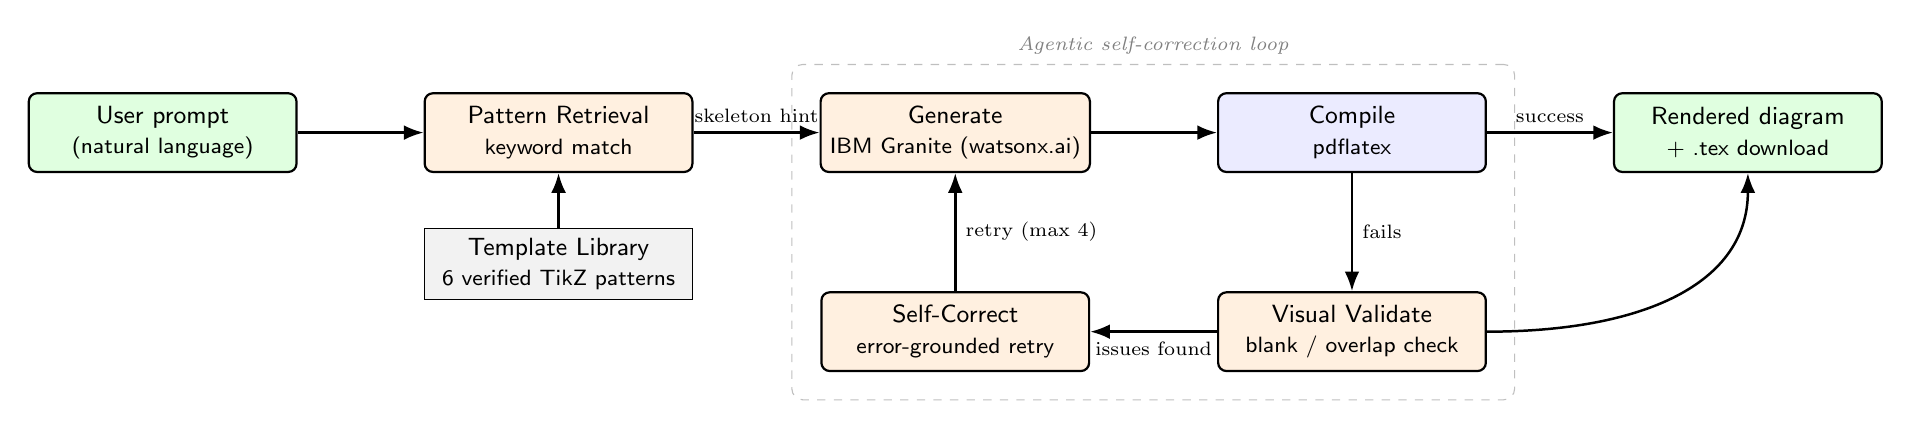
\begin{tikzpicture}[
  font=\sffamily\small,
  box/.style={rectangle, draw, rounded corners=3pt, minimum width=3.4cm, minimum height=1cm, align=center, fill=blue!8, line width=0.8pt},
  agent/.style={box, fill=orange!12},
  store/.style={rectangle, draw, minimum width=3.4cm, minimum height=0.9cm, align=center, fill=gray!10},
  arr/.style={-{Latex[length=2.5mm]}, line width=0.9pt}
]

\node[box, fill=green!12] (user) {User prompt\\ \footnotesize (natural language)};
\node[agent, right=1.6cm of user] (retrieve) {Pattern Retrieval\\ \footnotesize keyword match};
\node[store, below=0.7cm of retrieve] (lib) {Template Library\\ \footnotesize 6 verified TikZ patterns};
\node[agent, right=1.6cm of retrieve] (generate) {Generate\\ \footnotesize IBM Granite (watsonx.ai)};
\node[box, right=1.6cm of generate] (compile) {Compile\\ \footnotesize pdflatex};
\node[agent, below=1.5cm of compile] (validate) {Visual Validate\\ \footnotesize blank / overlap check};
\node[box, fill=green!12, right=1.6cm of compile] (out) {Rendered diagram\\ \footnotesize + .tex download};
\node[agent, below=1.5cm of generate] (fix) {Self-Correct\\ \footnotesize error-grounded retry};

\draw[arr] (user) -- (retrieve);
\draw[arr] (lib) -- (retrieve);
\draw[arr] (retrieve) -- node[above, font=\scriptsize]{skeleton hint} (generate);
\draw[arr] (generate) -- (compile);
\draw[arr] (compile) -- node[above, font=\scriptsize]{success} (out);
\draw[arr] (compile) -- node[right, font=\scriptsize]{fails} (validate);
\draw[arr] (validate) -- node[below, font=\scriptsize]{issues found} (fix);
\draw[arr] (fix) -- node[right, font=\scriptsize]{retry (max 4)} (generate);
\draw[arr] (validate.east) .. controls +(2,0) and +(0,-1.4) .. (out.south);

\begin{scope}[on background layer]
\node[draw=gray!50, dashed, rounded corners, fit=(generate)(compile)(validate)(fix), inner sep=10pt, label={[font=\scriptsize\itshape, gray]above:Agentic self-correction loop}] {};
\end{scope}

\end{tikzpicture}
\end{document}
